\section{Architektur}\label{Architektur}
\subsection{Struktur von SLD-Light}\label{SLD-Light}
Im Folgenden soll der Aufbau des neuen Dateiformats erläutert werden. Ein Beispiel ist in Listing \ref{lst:SLDLight} zu sehen. Die SLD-spezifischen Begriffe werden nicht im Detail erläutert\footnote{Erklärungen dafür können \cite{GeoServer_Doc} entnommen werden}. 

In der ersten Zeile der Datei steht der Name der \enquote{NamedLayer}. Darauf folgt die Angabe der Zoomstufen. Es müssen zwei Zahlen im Bereich von 0 bis 16 mit einem \enquote{-} voneinander getrennt angegeben werden. Die erste Zahl steht für die Mindestzoomstufe und die zweite Zahl für die Maximalzoomstufe, welche für die Regel gelten sollen. Die Stufen von 0 bis 16 werden vom Editor beim Übersetzen zu entsprechenden Werten übertragen, die für SLD geeignet sind. Die Stufeneinteilung kann Tabelle \ref{table:zoom} entnommen werden. Bei Angabe einer \enquote{0} wird die Angabe der Zoomstufe in der SLD-Datei weggelassen. 

Da eine Regel immer nur einen Zoom haben kann, folgt aus der Angabe der Zoomstufen, dass eine neue Regel begonnen wird. Aufgrund der niederen Wichtigkeit der Regelnamen gibt es keine Möglichkeit diesen in SLD-Light Dateien anzugeben. Der Regelname wird automatisch vergeben und setzt sich aus dem \enquote{NamedLayer}-Namen gefolgt \enquote{\textunderscore rule\textunderscore} und einem Index beginnend bei 0 zusammen.

Nach dem Zoom folgt eine optionale Angabe eines Filternamens. Dieser kann wichtig sein, wenn die Regel sich nur auf bestimmte Elemente der Karte beziehen soll.

Als Nächstes werden die sogenannten \enquote{Symbolizer} beschrieben. Diese bestimmen, wie die Objekte auf der Karte gezeichnet werden. Es gibt vier verschiedene Arten: PointSymbolizer, LineSymbolizer, PolygonSymbolizer und TextSymbolizer. Die Beschreibung im SLD-Light Format ist prinzipiell für alle gleich; zuerst wird der Typ angegeben und danach in runden Klammern die Eigenschaften, wobei die Reihenfolge dieser entscheidend ist. Im Folgenden wird die Reihenfolge der Eigenschaften beschrieben:

\begin{tabular}{l p{12cm}}
Punkt: & Point(wellKnownName, fillColor, size) \\

Linie: & Line(strokeColor, strokeWidth, strokeDashArray, perpendicularOffset) \\

Polygon: & Polygon(fillColor, fillOpacity, strokeColor, strokeWidth, strokeDashArray) \\

Text: & Text(label, fontSize, fontWeight, fill, anchorPointX, anchorPointY, displacementX, displacementY) \\
\end{tabular}

Weitere Regeln können hinzugefügt werden, indem weitere Angaben über Zoomstufen erfolgen. Dann ist klar, dass eine neue Regel angefangen wird und es können wieder Filter und Symbolizer hinzugefügt werden. 

\subsection{Aufbau des Editors}
Das Hauptfenster des Editors besteht aus zwei Bereichen. Auf der linken Seite befindet sich eine grafische Benutzeroberfläche, mit dessen Hilfe die Eigenschaften für die SLD-Datei eingestellt werden können. Auf der rechten Seite werden die aus diesen Eigenschaften erstellten Dateien angezeigt (siehe Abbildung \ref{abb:editor}). 

Beim Starten der Anwendung sind alle Bereiche weitestgehend leer. Um eine neue Regel hinzuzufügen klickt man auf den \enquote{Regel hinzufügen}-Button. Daraufhin werden vom Editor die Felder für \enquote{min Zoom}, \enquote{max Zoom}, \enquote{Filter} sowie ein Dropdown-Menü für Symbolizer angezeigt. Um einen Symbolizer hinzuzufügen, muss man den Typ in dem Dropdown-Menü auswählen und auf \enquote{Objekt hinzufügen} klicken. Der Editor schränkt den Benutzer aber insofern ein, dass für jede Regel nur jeweils ein Symbolizer eines bestimmten Typs hinzugefügt werden kann. Dies ist beabsichtigt, weil es prinzipiell wenig Sinn macht, in einer Regel zwei Symbolizer des gleichen Typs zu verwenden. 
Sobald ein Symbolizer hinzugefügt wurde, werden Eingabefelder mit den entsprechenden Eigenschaften erstellt und angezeigt. Für die Auswahl von Farben werden \enquote{ColorPicker}-Dialoge von JavaFX benutzt, damit der Benutzer nicht direkt mit den RGB-Farbcodes arbeiten muss. 

Links neben jedem Symbolizer wird ein \enquote{Löschen}-Button angezeigt, welcher die Eingabefelder wieder entfernt. Um eine ganze Regel zu entfernen, muss man auf den \enquote{Regel löschen}-Button, welcher sich rechts neben jeder Regel befindet, drücken.

Die Oberfläche besteht aus einer Verschachtelung von JavaFX-\enquote{GridPanes}\footnote{Layout, welches das Anordnen von Elementen in einem Raster, ermöglicht}. Beim Hinzufügen neuer Elemente wird in die passende Rasterzelle eine neue \enquote{GridPane} eingefügt, welche die neuen Eingabefelder zur Verfügung stellt. Damit ist die Benutzeroberfläche sehr flexibel und kann sich gut an Änderungen anpassen.

Im \enquote{Datei}-Reiter der Menüleiste finden sich vier Einträge, welche es ermöglichen den Editor zurückzusetzen, eine SLD-Light-Datei zu öffnen und die aktuelle Sitzung als SLD- oder SLD-Light-Datei abzuspeichern. Unter dem \enquote{Server}-Reiter der Menüleiste gibt es nur einen Eintrag, der ein neues Fenster öffnet, welches Dateiupload auf den Geoserver ermöglicht. Hier kann eine SLD-Datei und ein Workspace ausgewählt werden und durch einen Klick auf den \enquote{Hochladen}-Button wird diese Datei auf den Geoserver hochgeladen, sofern dieser erreicht werden kann (Hinweise dazu in Abschnitt \ref{Deployment}). Es stehen drei verschiedene Workspaces zur Verfügung: \enquote{PRODUCTION}, \enquote{TEST} und \enquote{DEFAULT}. Diese entscheiden, in welches Verzeichnis die Datei auf dem Geoserver abgelegt wird.


\subsection{Struktur der Objekte}

\begin{figure}[h]
 \centering
 \includegraphics[height=7in]{abb/uml}
 \caption{UML Diagramm: SLD-Objekte}\label{abb:uml}
\end{figure}

Die Architektur der Objekte, welche die Daten über eine SLD-Layer enthalten, ist in Abbildung \ref{abb:uml} dargestellt. Jedes Objekt implementiert das \enquote{SLDObject}-Interface und muss damit Implementierungen für die Methoden \enquote{toSLD()} und \enquote{toSLDLight()} bereitstellen. Die Symbolizer-Objekte implementieren das Marker-Interface \enquote{Symbolizer}. Damit wird sichergestellt, dass zur Liste im \enquote{Regel}-Objekt nur Symbolizer-Objekte und keine anderen SLD-Objekte hinzugefügt werden können. 

Das Erzeugen der Inhalte für SLD und SLD-Light erfolgt über Aufrufe der SLDObject-Methoden \enquote{toSLD()} bzw. \enquote{toSLDLight()}. Das \enquote{NamedLayer} Objekt benutzt die Ergebnisse der SLDObject-Methoden der \enquote{Regel}-Objekte und die \enquote{Regel}-Objekte benutzen die Ergebnisse der SLDObject-Methoden der Symbolizer, welche in ihrer Liste stehen. So wird rekursiv das Endergebnis erzeugt. 

Jedes SLD-Objekt hat einen Konstruktor, der einen String Parameter erwartet. Diese Zeichenkette muss die Definition des jeweiligen Objektes in SLD-Light-Kodierung beinhalten. Ein \enquote{LineSymbolizer} würde im Konstruktor zum Beispiel so etwas wie \enquote{Line(\#CCCCCC, 2, 5 2, 3)} erwarten und die eigenen Attribute daraus ableiten. 

\subsection{Dateiupload}

\begin{figure}[h]
 \centering
 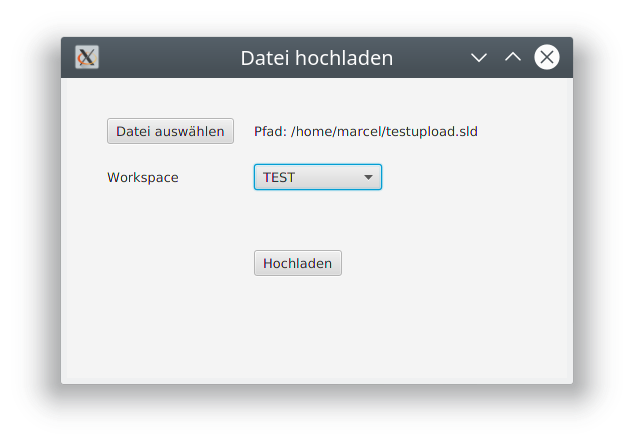
\includegraphics[width=0.5\textwidth]{abb/dateiupload}
 \caption{Dateiupload-Fenster}\label{abb:dateiupload}
\end{figure}

Der Editor ermöglicht es dem Benutzer eine SLD-Datei und einen Workspace auszuzuwählen, in welchen die Datei platziert werden soll (siehe Abbildung \ref{abb:dateiupload}). Hierbei ist anzumerken, dass der Upload der SLD-Datei nicht ausreicht, da der Geoserver auf weitere Informationen in einer weiteren XML-Datei zurückgreift. Die XML-Datei wird von der Anwendung zusätzlich erzeugt und muss den gleichen Namen (bis auf die Dateiendung), wie die SLD-Datei haben. Ein Beispiel kann in Listing \ref{lst:XML_SLD} betrachtet werden. 

Die Workspace-ID kann XML-Dateien, welche sich auf dem Geoserver befinden, entnommen werden. Sie steht in der \enquote{workspace.xml}-Datei, welche sich in jedem Workspace-Verzeichnis befindet. Es ist unklar, wie sich die Style-ID zusammensetzt. Zwischen den XML-Dateien im gleichen Workspace unterscheidet sich bei dieser ID nur der Teil hinter dem letzten Doppelpunkt, was auf einen internen Nummerierungsmechanismus hindeutet. Die entwickelte Anwendung verwendet momentan bei einem Upload immer die gleiche Style-ID. Unerwünschte Folgen davon sind nicht bekannt, aber nicht auszuschließen.  

\subsection{Genutzte Komponenten}
Zur Erstellung einer Verbindung mit dem OHDM-Server wird die \enquote{sshj}-Bibliothek\footnote{Projektseite: \url{https://github.com/hierynomus/sshj/tree/master}} genutzt. Diese ermöglicht es \enquote{ssh}-, \enquote{scp}- und \enquote{sftp}-Verbindungen in Java zu erzeugen. In der entwickelten Anwendung werden nur SFTP-Verbindungen benötigt. Die anderen Dateien, welche sich im \enquote{lib}-Ordner des Projektes befinden, sind Abhängigkeiten, welche für die korrekte Ausführung der \enquote{sshj}-Bibliothek benötigt werden. 
Aktuelle Releases der Bibliothek können von der GitHub-Seite des Projektes heruntergeladen oder über Maven in das Projekt eingebunden werden. Die Einbindung wird auf der Projektseite detailliert erklärt.